\chapter{Results and Empirical Analysis\label{cha:chapter5}}

Because of the varying stability of prompt effects across code/math and local/API settings, the results are organized by task type and model group. The local and API groups are complementary experiments run under different models, task datasets, and serving environments, so cross-group differences are reported descriptively and are not interpreted as head-to-head model comparisons. Model ability is generally more determinative of whether an answer is correct, while prompt framing is more determinative of observable behavior than of functional correctness.

This chapter is organized to answer the four research questions in turn. Section~\ref{sec:data-integrity} verifies data integrity. Section~\ref{sec:model-ability-dominates} answers RQ1 by comparing model and prompt effect sizes. Sections~\ref{sec:code-task-effects}--\ref{sec:mixed-effects-results} answer RQ2 on correctness, moving from descriptive contrasts to the main mixed-effects inference. Section~\ref{sec:output-behavior} answers RQ3 on observable behavior. Section~\ref{sec:mediation-results} answers RQ4 on behavior-adjusted contrasts. Sections~\ref{sec:lpm-robustness}--\ref{sec:dominant-sensitivity} report robustness and aggregation risk, and Section~\ref{sec:failure-modes} summarizes failure modes. Table~\ref{tab:key-findings} gives the key findings at a glance before the detailed subsections.

\begin{longtable}[]{@{}
 >{\raggedright\arraybackslash}p{(\linewidth - 6\tabcolsep) * \real{0.16}}
 >{\raggedright\arraybackslash}p{(\linewidth - 6\tabcolsep) * \real{0.38}}
 >{\raggedright\arraybackslash}p{(\linewidth - 6\tabcolsep) * \real{0.30}}
 >{\raggedright\arraybackslash}p{(\linewidth - 6\tabcolsep) * \real{0.16}}@{}}
\caption{Key findings at a glance. Correctness effects are mixed-effects average marginal effects in percentage points; behavior effects are percent changes unless marked pp.}\label{tab:key-findings}\tabularnewline
\toprule\noalign{}
Stratum & Correctness (pass/fail) & Output behavior & Details \\
\midrule\noalign{}
\endfirsthead
\toprule\noalign{}
Stratum & Correctness (pass/fail) & Output behavior & Details \\
\midrule\noalign{}
\endhead
\bottomrule\noalign{}
\endlastfoot
Local code & Small role penalty (-1.0 pp); tone and format null & Polite tone: +12.4\% tokens, +10.8\% duration; JSON/XML improve compliance & Sec. \ref{sec:code-task-effects}, \ref{sec:mixed-effects-results}, \ref{sec:output-behavior} \\
Local math & JSON penalty -4.1 pp, XML penalty -2.1 pp; role +2.1 pp and polite +1.6 pp gains & JSON: -19.8\% tokens; polite tone: +11.0\% tokens & Sec. \ref{sec:math-task-effects}, \ref{sec:mixed-effects-results} \\
API Python & JSON gain +3.4 pp, XML gain +5.2 pp & Wrappers reduce tokens and duration & Sec. \ref{sec:code-task-effects}, \ref{sec:mixed-effects-results} \\
API math & Role penalty -2.8 pp & Role framing: +83 tokens & Sec. \ref{sec:math-task-effects}, \ref{sec:mixed-effects-results} \\
Sensitivity & Local effects survive Nemotron removal; API Python effects attenuate without DeepSeek & -- & Sec. \ref{sec:dominant-sensitivity} \\
\end{longtable}

\section{Data Integrity and Run Coverage\label{sec:data-integrity}}

The Consolidated Results Package includes 12 local JSONL files and four API JSONL files. Each model-task file contains 900 records, and there are no duplicate full run keys. Each base task contains all 18 prompt variants for each model-task combination. No gaps were found in the prompt metadata join. Empty responses are rare: there are only 14 in the Local Results Package (all in the Nemotron code outputs) and zero in the API Results Package. The data-integrity and run-coverage verification results are detailed in Table~\ref{tab:data-integrity}.

\begin{longtable}[]{@{}ll@{}}
\caption{Data-integrity and run-coverage checks.}\label{tab:data-integrity}\tabularnewline
\toprule\noalign{}
Check & Result \\
\midrule\noalign{}
\endfirsthead
\toprule\noalign{}
Check & Result \\
\midrule\noalign{}
\endhead
\bottomrule\noalign{}
\endlastfoot
Local result files & 12 JSONL files, 900 rows each \\
API result files & 4 JSONL files, 900 rows each \\
Duplicate task keys & 0 \\
Prompt metadata join gaps & 0 \\
Empty local responses & 14, all Nemotron code \\
Empty API responses & 0 \\
\end{longtable}

\section{Model Ability Dominates Correctness\label{sec:model-ability-dominates}}

Model choice has a much larger effect than prompt-factor choice. Figure~\ref{fig:model_performance_by_task} shows that local code pass rates range from 0.4\% to 22.8\%, local math from 5.7\% to 91.2\%, API Python from 66.7\% to 69.0\%, and API math from 24.1\% to 82.4\%. The model-level pass rates, median durations, and completion token counts are presented in Table~\ref{tab:model-pass-rates}.

\begin{figure}[htbp]
\centering
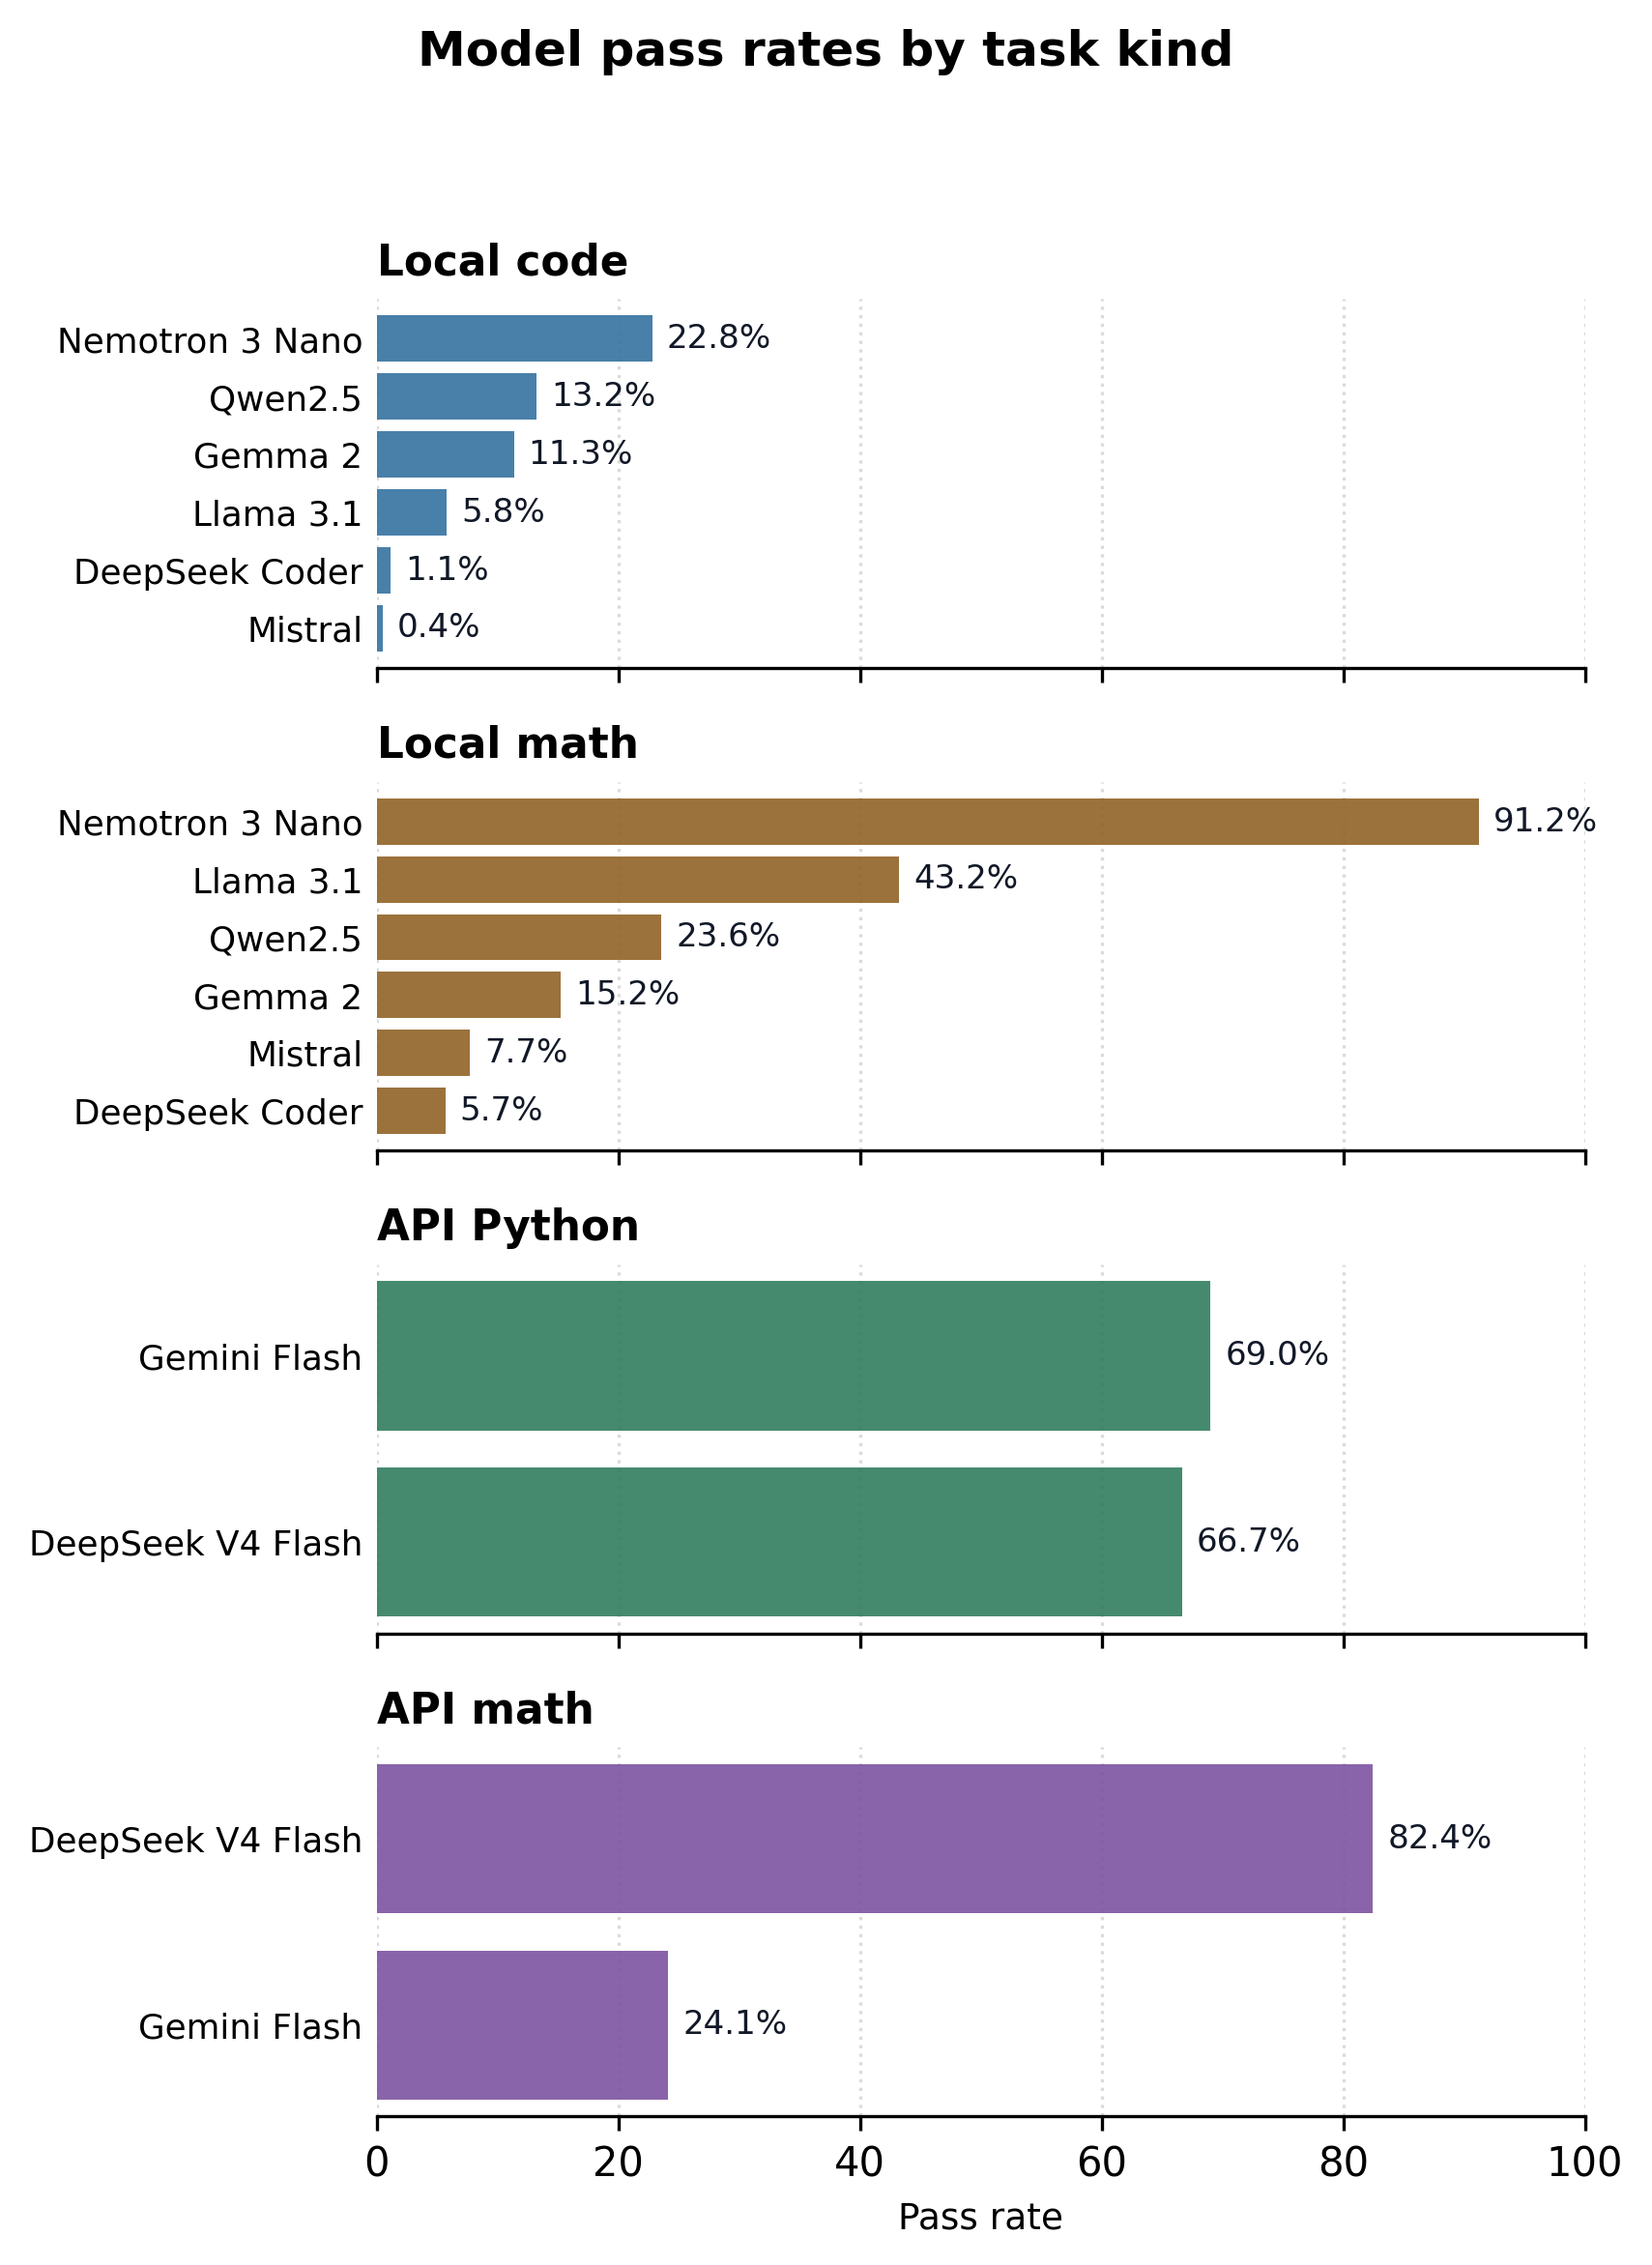
\includegraphics[width=0.95\linewidth,height=\textheight,keepaspectratio,alt={Model pass rates by task kind. The figure highlights that between-model variation is larger than the main prompt-factor effects reported in later sections.}]{figures/model_performance_by_task.png}
\caption{Model pass rates by task kind. The figure highlights that between-model variation is larger than the main prompt-factor effects reported in later sections.}
\label{fig:model_performance_by_task}
\end{figure}

\begin{longtable}[]{@{}
 >{\raggedright\arraybackslash}p{(\linewidth - 8\tabcolsep) * \real{0.1667}}
 >{\raggedright\arraybackslash}p{(\linewidth - 8\tabcolsep) * \real{0.1667}}
 >{\raggedleft\arraybackslash}p{(\linewidth - 8\tabcolsep) * \real{0.2222}}
 >{\raggedleft\arraybackslash}p{(\linewidth - 8\tabcolsep) * \real{0.2222}}
 >{\raggedleft\arraybackslash}p{(\linewidth - 8\tabcolsep) * \real{0.2222}}@{}}
\caption{Model-level pass rates and output behavior.}\label{tab:model-pass-rates}\tabularnewline
\toprule\noalign{}
\begin{minipage}[b]{\linewidth}\raggedright
Task kind
\end{minipage} & \begin{minipage}[b]{\linewidth}\raggedright
Model
\end{minipage} & \begin{minipage}[b]{\linewidth}\raggedleft
Pass rate
\end{minipage} & \begin{minipage}[b]{\linewidth}\raggedleft
Median duration
\end{minipage} & \begin{minipage}[b]{\linewidth}\raggedleft
Mean completion tokens
\end{minipage} \\
\midrule\noalign{}
\endfirsthead
\toprule\noalign{}
\begin{minipage}[b]{\linewidth}\raggedright
Task kind
\end{minipage} & \begin{minipage}[b]{\linewidth}\raggedright
Model
\end{minipage} & \begin{minipage}[b]{\linewidth}\raggedleft
Pass rate
\end{minipage} & \begin{minipage}[b]{\linewidth}\raggedleft
Median duration
\end{minipage} & \begin{minipage}[b]{\linewidth}\raggedleft
Mean completion tokens
\end{minipage} \\
\midrule\noalign{}
\endhead
\bottomrule\noalign{}
\endlastfoot
local code & nemotron-3-nano-4b & 22.8\% & 17.78s & 1646 \\
local code & qwen2.5-7b & 13.2\% & 8.75s & 316 \\
local code & gemma2-9b & 11.3\% & 5.52s & 175 \\
local code & llama3.1-8b & 5.8\% & 11.16s & 394 \\
local code & deepseek-coder-6.7b & 1.1\% & 9.04s & 491 \\
local code & mistral-7b-instruct & 0.4\% & 9.12s & 366 \\
local math & nemotron-3-nano-4b & 91.2\% & 3.15s & 289 \\
local math & llama3.1-8b & 43.2\% & 5.09s & 274 \\
local math & qwen2.5-7b & 23.6\% & 0.68s & 6 \\
local math & gemma2-9b & 15.2\% & 0.80s & 6 \\
local math & mistral-7b-instruct & 7.7\% & 0.89s & 79 \\
local math & deepseek-coder-6.7b & 5.7\% & 5.35s & 287 \\
API Python & gemini-flash & 69.0\% & 10.30s & 359 \\
API Python & deepseek-v4-flash & 66.7\% & 16.12s & 1352 \\
API math & deepseek-v4-flash & 82.4\% & 9.41s & 1127 \\
API math & gemini-flash & 24.1\% & 3.40s & 15 \\
\end{longtable}

The differences between the various models are much greater than the differences between the prompt variants. For instance, the local math gap between Nemotron and DeepSeek Coder is 85.5 percentage points, and the greatest pooled local prompt format effect is 4.2 percentage points.

This establishes the scale for the rest of the results: prompt factors are secondary to much larger model and task differences, but still meaningful. A prompt-policy recommendation that ignores the actual model is misleading. The practical question is not whether better prompting can make a weak model perform like a strong one; the evidence does not support that. The useful question is whether better framing makes the chosen model work more smoothly with the evaluator, cost less to run, and fail in fewer, more predictable ways.

\section{Prompt-Factor Effects on Code Tasks\label{sec:code-task-effects}}

The pooled results for local code tasks show no significant tone or format effects on correctness. The pass rate for both neutral and aggressive prompts is 9.3\%, while the pass rate for polite prompts is 8.8\%. Role framing reduces the pass rate slightly (from 9.6\% to 8.6\%); the raw pooled contrast is not significant, but the mixed-effects and clustered models both support a small role penalty of about one percentage point. XML shows a slight advantage over plaintext and JSON, but the differences are small and not statistically significant. The prompt-factor contrasts for local code tasks are summarized in Table~\ref{tab:local-code-contrasts}.

\begin{longtable}[]{@{}llrrrr@{}}
\caption{Local code prompt-factor contrasts.}\label{tab:local-code-contrasts}\tabularnewline
\toprule\noalign{}
Factor & Contrast & Pass diff & p & Token diff & Duration diff \\
\midrule\noalign{}
\endfirsthead
\toprule\noalign{}
Factor & Contrast & Pass diff & p & Token diff & Duration diff \\
\midrule\noalign{}
\endhead
\bottomrule\noalign{}
\endlastfoot
tone & aggressive vs neutral & +0.0 pp & 1.000 & +4 & +0.10s \\
tone & polite vs neutral & -0.5 pp & 0.601 & +30 & +0.96s \\
role & role vs none & -1.0 pp & 0.185 & +15 & +0.27s \\
format & JSON vs plaintext & +0.2 pp & 0.860 & -16 & -0.39s \\
format & XML vs plaintext & +0.8 pp & 0.387 & -21 & -0.46s \\
\end{longtable}

For local code tasks, the results are more strongly behavior-based than correctness-based. Completion tokens and duration increase when polite prompts are used, but this does not impact the overall pass rate. Role prompts also increase verbosity. Using JSON/XML decreases the number of tokens and duration while achieving a higher level of result-only/code-only compliance. Ultimately, the behavioral gains driven by prompt usage do not result in meaningful improvements in the pooled pass rate for local code.

In API Python, JSON raises the raw pass rate by 3.2 percentage points while reducing token count by 105 and request time by 1.55 seconds. Similarly, XML raises the pass rate by 4.8 percentage points while reducing tokens by 77 and duration by 1.12 seconds. The raw two-proportion p-values fail to reach the 0.05 significance threshold, but the clustered fixed-effect p-values do. As a result, XML remains statistically significant, while JSON is positive but marginal. The prompt-format contrasts for API Python tasks are shown in Table~\ref{tab:api-python-contrasts}.

\begin{longtable}[]{@{}llrrrr@{}}
\caption{API Python prompt-format contrasts.}\label{tab:api-python-contrasts}\tabularnewline
\toprule\noalign{}
Factor & Contrast & Pass diff & p & Token diff & Duration diff \\
\midrule\noalign{}
\endfirsthead
\toprule\noalign{}
Factor & Contrast & Pass diff & p & Token diff & Duration diff \\
\midrule\noalign{}
\endhead
\bottomrule\noalign{}
\endlastfoot
format & JSON vs plaintext & +3.2 pp & 0.244 & -105 & -1.55s \\
format & XML vs plaintext & +4.8 pp & 0.074 & -77 & -1.12s \\
\end{longtable}

This comparison has important implications for engineering interpretation. Structured wrappers can assist coding workflows when they enhance parser compatibility and decrease unnecessary output, but this benefit does not apply universally across all model groups or task types.

The API Python result was the strongest positive finding for structured wrappers in this experiment, especially when considering the clustered robustness check. This result is also limited to two hosted models, one Python task family, and a very strict code-only system prompt. Consequently, it may be worthwhile to try using JSON or XML wrappers in the coding workflows of API-based development; this will be most beneficial when downstream tooling benefits from compact task boundaries. However, this study does not support applying the same wrapper policy across all model groups or task types.

\section{Prompt-Factor Effects on Math Tasks\label{sec:math-task-effects}}

Analysis of the data shows that math tasks are more sensitive to prompt framing at the model-specific level than code tasks are. At the local level, using JSON reduces the pooled pass rate by 4.2 percentage points and decreases both tokens used and duration. Using XML reduces the pooled pass rate by 2.2 percentage points, though the unadjusted statistical contrast is not significant. Using role framing also has a positive, but marginal, effect on local math. The prompt-factor contrasts for local math tasks are listed in Table~\ref{tab:local-math-contrasts}.

\begin{longtable}[]{@{}llrrrr@{}}
\caption{Local math prompt-factor contrasts.}\label{tab:local-math-contrasts}\tabularnewline
\toprule\noalign{}
Factor & Contrast & Pass diff & p & Token diff & Duration diff \\
\midrule\noalign{}
\endfirsthead
\toprule\noalign{}
Factor & Contrast & Pass diff & p & Token diff & Duration diff \\
\midrule\noalign{}
\endhead
\bottomrule\noalign{}
\endlastfoot
tone & aggressive vs neutral & +0.9 pp & 0.539 & +7 & +0.29s \\
tone & polite vs neutral & +1.7 pp & 0.280 & +17 & +0.55s \\
role & role vs none & +2.2 pp & 0.083 & +11 & +0.29s \\
format & JSON vs plaintext & -4.2 pp & 0.007 & -32 & -0.92s \\
format & XML vs plaintext & -2.2 pp & 0.153 & +1 & -0.02s \\
\end{longtable}

Only some models are adversely affected by the local math format effect, as indicated by separate model analyses. Llama 3.1 dropped 15.7 percentage points under JSON and 9.7 percentage points under XML, while DeepSeek Coder dropped 4.3 percentage points under JSON and 5.7 percentage points under XML. The Qwen 2.5 model benefited from role framing, with an increase of 10.2 percentage points. The mixed results indicate that the ultimate conclusion is not that "JSON is bad"; rather, it is that "format effects are model- and task-dependent."

An analysis using the Benjamini-Hochberg correction procedure applied to the 60 local baseline contrasts supports a cautious interpretation of the results. Seven of the 60 have an uncorrected p-value \textless{} 0.05; however, after treating all 60 as one family, only two remain statistically significant: Llama 3.1's JSON penalty in math and Qwen 2.5's role-framing gain in math. When the code and math conditions are treated as two different families of 30 each, there are no remaining significant results for code, but there are 3 significant results for math: Llama 3.1 JSON, Qwen 2.5 role framing, and DeepSeek Coder XML. Therefore, the results of this analysis support the conclusion that sensitivity to prompt types is more of a phenomenon related to the math side of the dataset than the coding side.

For API math, role framing shows a small negative effect: it decreases the pass rate by 2.8 percentage points and increases tokens by 83. The raw comparison is not statistically significant; however, the clustered model check verified that the negative direction remains evident. The role-framing contrast for API math tasks is detailed in Table~\ref{tab:api-math-contrast}.

\begin{longtable}[]{@{}llrrrr@{}}
\caption{API math role-framing contrast.}\label{tab:api-math-contrast}\tabularnewline
\toprule\noalign{}
Factor & Contrast & Pass diff & p & Token diff & Duration diff \\
\midrule\noalign{}
\endfirsthead
\toprule\noalign{}
Factor & Contrast & Pass diff & p & Token diff & Duration diff \\
\midrule\noalign{}
\endhead
\bottomrule\noalign{}
\endlastfoot
role & role vs none & -2.8 pp & 0.238 & +83 & +0.47s \\
\end{longtable}

The combined math analyses answer RQ2 and RQ3 more robustly than pooling the individual math tables alone. The direction of format and role effects varies based on the model used and the task type. The math penalties observed with local JSON formatting serve as a cautionary reminder not to assume that structured wrappers will always improve performance. The Qwen role gain and the API role penalty confirm this for persona prompts; that is, framing a question with a role can increase the pass rate, decrease it, or mainly change the verbosity of the output depending on the model and evaluator.

\section{Mixed-Effects Inferential Results\label{sec:mixed-effects-results}}

Table~\ref{tab:mixed-effects-pass} reports the main inferential analysis: mixed-effects logistic models for pass/fail including prompt-factor and model fixed effects and a random intercept per base task, fitted per stratum. The average marginal effects are expressed in percentage points so they can be read alongside the descriptive contrast tables above.

{\small
\setlength{\tabcolsep}{4pt}
\begin{longtable}[]{@{}llrrr@{}}
\caption{Mixed-effects logistic results for pass/fail by stratum: odds ratios and average marginal effects (AME) in percentage points, with 95\% intervals and posterior p-values.}\label{tab:mixed-effects-pass}\tabularnewline
\toprule\noalign{}
Stratum & Contrast & Odds ratio [95\% int.] & AME pp [95\% int.] & p \\
\midrule\noalign{}
\endfirsthead
\toprule\noalign{}
Stratum & Contrast & Odds ratio [95\% int.] & AME pp [95\% int.] & p \\
\midrule\noalign{}
\endhead
\bottomrule\noalign{}
\endlastfoot
API Python & Aggressive tone & 1.05 [0.83, 1.34] & +0.6 [-2.3, +3.4] & 0.686 \\
API Python & Polite tone & 1.05 [0.83, 1.34] & +0.6 [-2.2, +3.4] & 0.686 \\
API Python & Role framing & 0.92 [0.76, 1.11] & -1.1 [-3.5, +1.2] & 0.381 \\
API Python & JSON wrapper & 1.32 [1.04, 1.68] & +3.4 [+0.5, +6.2] & 0.022 \\
API Python & XML wrapper & 1.55 [1.21, 1.97] & +5.2 [+2.4, +8.0] & \textless{}0.001 \\
API math & Aggressive tone & 1.05 [0.81, 1.38] & +0.5 [-2.1, +2.9] & 0.697 \\
API math & Polite tone & 0.91 [0.70, 1.18] & -0.9 [-3.5, +1.5] & 0.476 \\
API math & Role framing & 0.74 [0.60, 0.92] & -2.8 [-4.8, -0.8] & 0.006 \\
API math & JSON wrapper & 0.87 [0.67, 1.14] & -1.3 [-3.8, +1.2] & 0.325 \\
API math & XML wrapper & 0.78 [0.60, 1.02] & -2.3 [-4.7, +0.1] & 0.069 \\
Local code & Aggressive tone & 0.98 [0.80, 1.20] & -0.1 [-1.0, +0.9] & 0.858 \\
Local code & Polite tone & 0.89 [0.72, 1.09] & -0.5 [-1.4, +0.4] & 0.265 \\
Local code & Role framing & 0.81 [0.68, 0.96] & -1.0 [-1.7, -0.2] & 0.013 \\
Local code & JSON wrapper & 1.01 [0.83, 1.24] & +0.1 [-0.8, +1.0] & 0.900 \\
Local code & XML wrapper & 1.15 [0.94, 1.41] & +0.7 [-0.2, +1.6] & 0.164 \\
Local math & Aggressive tone & 1.11 [0.95, 1.29] & +0.9 [-0.5, +2.2] & 0.198 \\
Local math & Polite tone & 1.20 [1.03, 1.40] & +1.6 [+0.3, +3.0] & 0.019 \\
Local math & Role framing & 1.28 [1.13, 1.45] & +2.1 [+1.0, +3.2] & \textless{}0.001 \\
Local math & JSON wrapper & 0.62 [0.52, 0.72] & -4.1 [-5.4, -2.8] & \textless{}0.001 \\
Local math & XML wrapper & 0.78 [0.66, 0.91] & -2.1 [-3.4, -0.9] & 0.001 \\
\end{longtable}
}

According to the mixed-effects results, all of the headline findings are confirmed. The results of the main inferential analysis confirm the benefit of the structured format in API Python code for both JSON (OR 1.32, p = 0.022) and XML (OR 1.55, p \textless{} 0.001). The penalty for local math in JSON is clearly established (OR 0.62, p \textless{} 0.001); the penalty for local math in XML is also confirmed (OR 0.78, p = 0.001), as are the gain from local math in role-framing (OR 1.28, p \textless{} 0.001) and the small polite-tone gain in local math (OR 1.20, p = 0.019). The role-framing penalty in API math, which was regarded as exploratory in the descriptive analysis, was confirmed in the mixed model (OR 0.74, p = 0.006). The small penalty for the local-code role is also confirmed in the mixed analysis (OR 0.81, p = 0.013); however, at roughly one percentage point, it remains practically minor. No tone effects can be regarded as significant in either code stratum.

The behavioral mixed models present the same findings as the descriptive behavior tables. Using linear mixed models with random task-specific intercepts, polite language leads to an increase in log completion tokens and log duration in the local strata, while the use of both JSON and XML decreases these figures; additionally, role framing modestly increases them. These overall effect directions confirm what is seen in the descriptive behavior tables. Furthermore, the result-only compliance outcome remains constant for API code under strict system prompts, meaning no compliance model can be estimated in that context.

\section{Output Behavior: Tokens, Duration, and Compliance\label{sec:output-behavior}}

Prompt framing changes observable output behavior more reliably than correctness. In the case of coding tasks, a polite tone leads to 12.40\% more completion tokens, a 7.00-percentage-point decline in result-only compliance, and an increase of 10.76\% in duration. Role framing results in 3.17\% more tokens and 2.41\% longer duration. JSON and XML reduce tokens and duration but improve result-only compliance.

Figure~\ref{fig:behavior-effects} visualizes these behavior effects, split by unit: panel (a) shows token and duration effects in percent, panel (b) shows result-only compliance effects in percentage points. The largest behavior changes are not always correctness gains: polite tone increases output length and duration, while JSON strongly shortens local math responses. The observable output behavior effects for local code tasks are presented in Table~\ref{tab:local-code-behavior}, and for local math tasks in Table~\ref{tab:local-math-behavior}.

\begin{figure}[htbp]
\centering
\begin{minipage}[b]{0.78\linewidth}
\centering
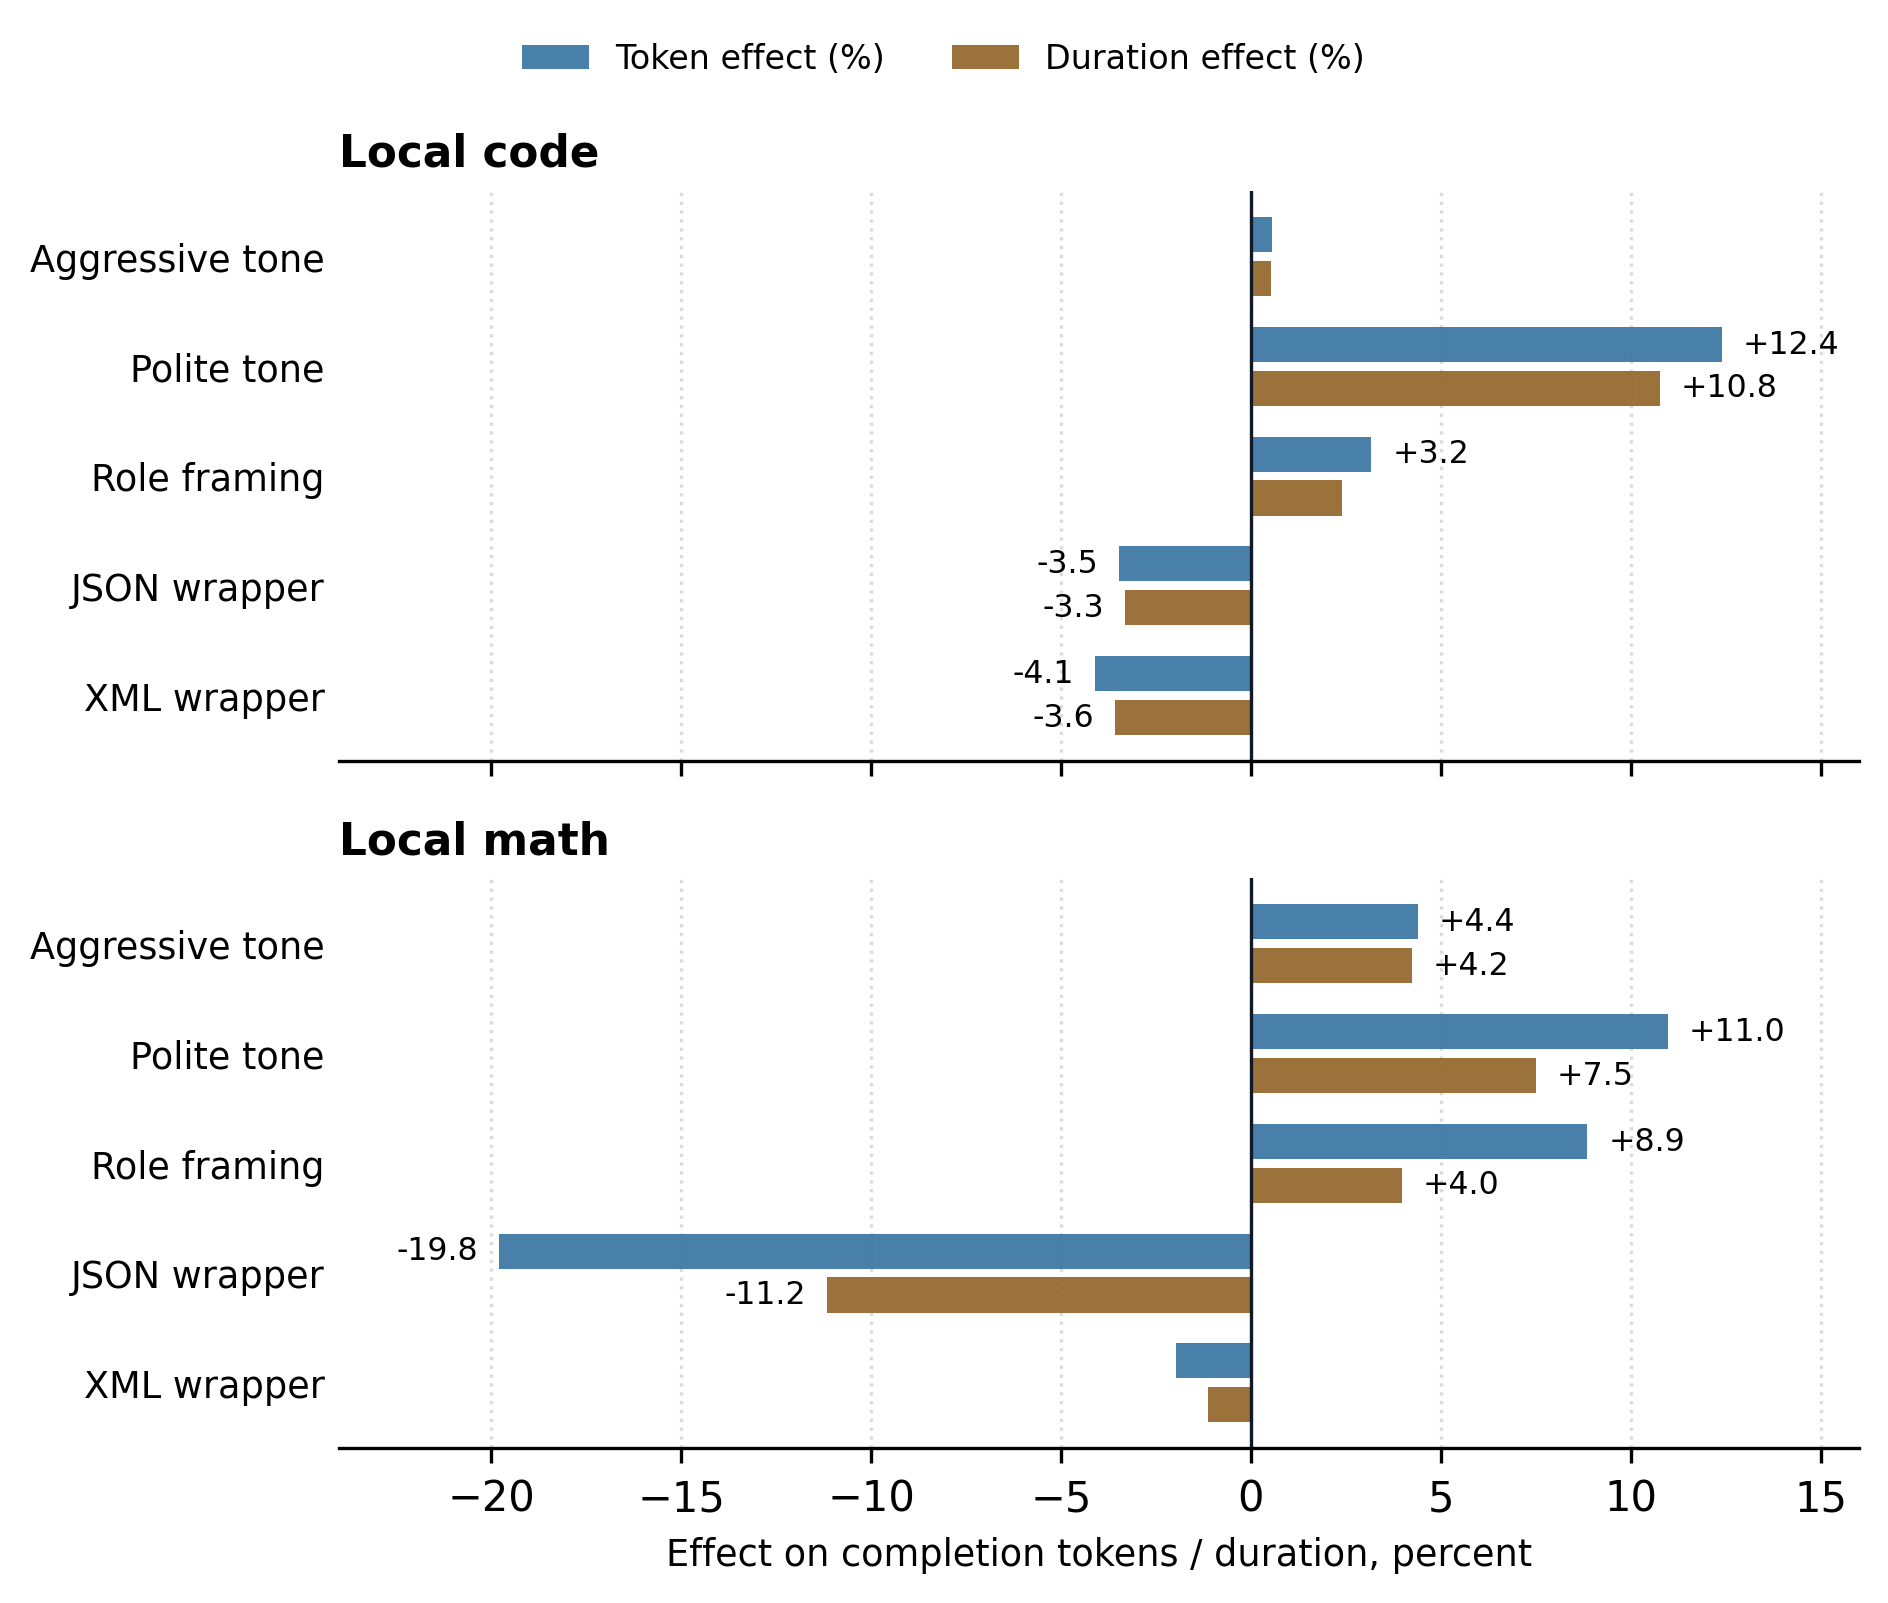
\includegraphics[width=\linewidth,alt={Token and duration effects in percent for local code and local math.}]{figures/behavior_effects_tokens_duration.png}
\centering\textbf{(a)} Token and duration effects, percent
\end{minipage}

\vspace{0.8em}

\begin{minipage}[b]{0.78\linewidth}
\centering
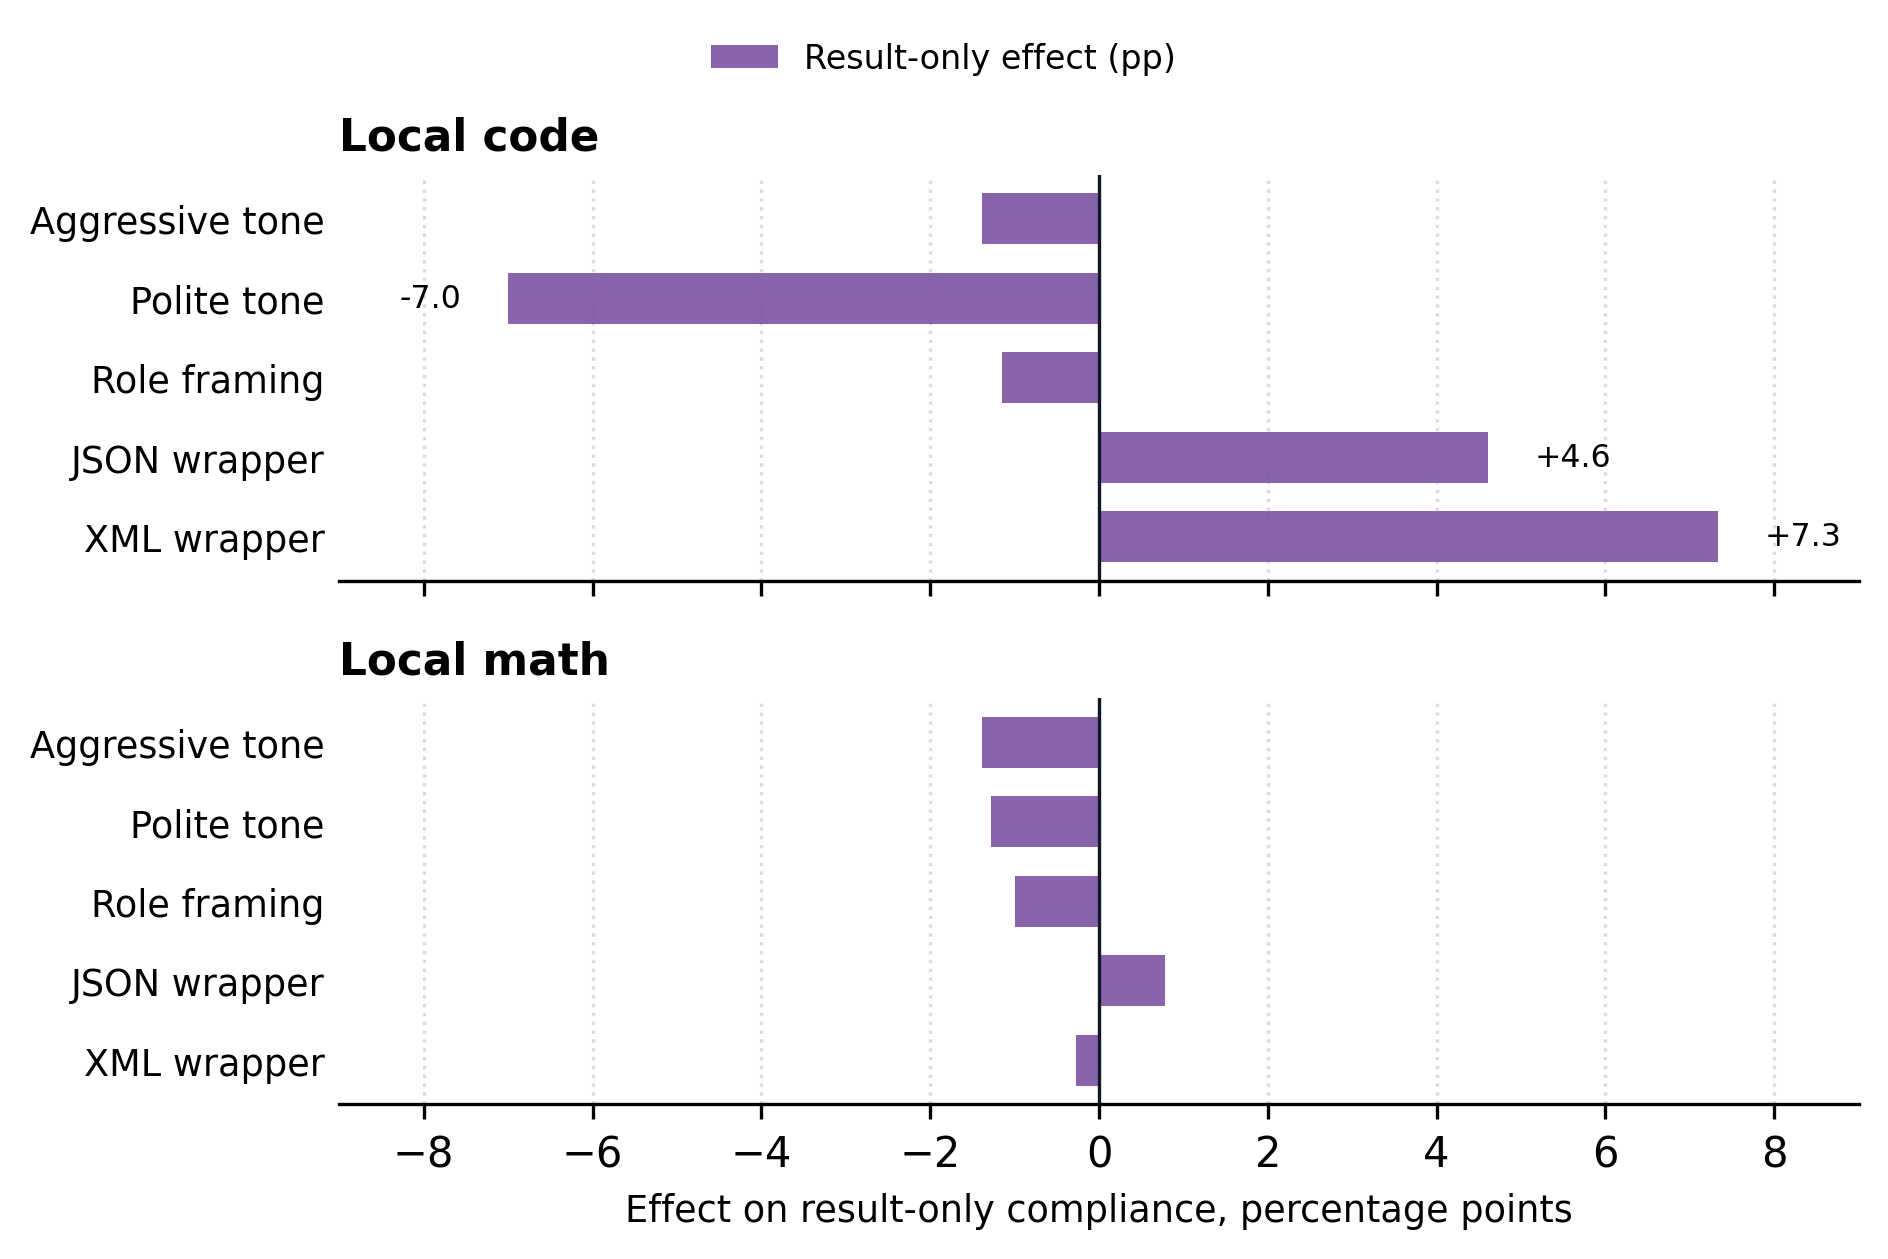
\includegraphics[width=\linewidth,alt={Result-only compliance effects in percentage points for local code and local math.}]{figures/behavior_effects_compliance.png}
\centering\textbf{(b)} Result-only compliance effects, percentage points
\end{minipage}
\caption{Prompt-factor effects on output behavior for local code and local math. Panel (a): effects on completion tokens and duration, in percent. Panel (b): effects on result-only compliance, in percentage points.}
\label{fig:behavior-effects}
\end{figure}

\begin{longtable}[]{@{}
 >{\raggedright\arraybackslash}p{(\linewidth - 6\tabcolsep) * \real{0.2000}}
 >{\raggedleft\arraybackslash}p{(\linewidth - 6\tabcolsep) * \real{0.2667}}
 >{\raggedleft\arraybackslash}p{(\linewidth - 6\tabcolsep) * \real{0.2667}}
 >{\raggedleft\arraybackslash}p{(\linewidth - 6\tabcolsep) * \real{0.2667}}@{}}
\caption{Local code behavior effects.}\label{tab:local-code-behavior}\tabularnewline
\toprule\noalign{}
\begin{minipage}[b]{\linewidth}\raggedright
Local code factor
\end{minipage} & \begin{minipage}[b]{\linewidth}\raggedleft
Token effect
\end{minipage} & \begin{minipage}[b]{\linewidth}\raggedleft
Result-only effect
\end{minipage} & \begin{minipage}[b]{\linewidth}\raggedleft
Duration effect
\end{minipage} \\
\midrule\noalign{}
\endfirsthead
\toprule\noalign{}
\begin{minipage}[b]{\linewidth}\raggedright
Local code factor
\end{minipage} & \begin{minipage}[b]{\linewidth}\raggedleft
Token effect
\end{minipage} & \begin{minipage}[b]{\linewidth}\raggedleft
Result-only effect
\end{minipage} & \begin{minipage}[b]{\linewidth}\raggedleft
Duration effect
\end{minipage} \\
\midrule\noalign{}
\endhead
\bottomrule\noalign{}
\endlastfoot
Aggressive tone & +0.55\% & -1.39 pp & +0.52\% \\
Polite tone & +12.40\% & -7.00 pp & +10.76\% \\
Role framing & +3.17\% & -1.15 pp & +2.41\% \\
JSON wrapper & -3.46\% & +4.61 pp & -3.32\% \\
XML wrapper & -4.10\% & +7.33 pp & -3.57\% \\
\end{longtable}

In math tasks, polite prompts increase tokens and duration, and role prompts do the same, but JSON strongly reduces both. Result-only compliance is also relatively unchanged for math tasks because the majority of models have stable response patterns regardless of the prompt. Typically, Qwen, Gemma, and Nemotron provide short responses, whereas Llama and DeepSeek provide lengthy responses.

\begin{longtable}[]{@{}
 >{\raggedright\arraybackslash}p{(\linewidth - 6\tabcolsep) * \real{0.2000}}
 >{\raggedleft\arraybackslash}p{(\linewidth - 6\tabcolsep) * \real{0.2667}}
 >{\raggedleft\arraybackslash}p{(\linewidth - 6\tabcolsep) * \real{0.2667}}
 >{\raggedleft\arraybackslash}p{(\linewidth - 6\tabcolsep) * \real{0.2667}}@{}}
\caption{Local math behavior effects.}\label{tab:local-math-behavior}\tabularnewline
\toprule\noalign{}
\begin{minipage}[b]{\linewidth}\raggedright
Local math factor
\end{minipage} & \begin{minipage}[b]{\linewidth}\raggedleft
Token effect
\end{minipage} & \begin{minipage}[b]{\linewidth}\raggedleft
Result-only effect
\end{minipage} & \begin{minipage}[b]{\linewidth}\raggedleft
Duration effect
\end{minipage} \\
\midrule\noalign{}
\endfirsthead
\toprule\noalign{}
\begin{minipage}[b]{\linewidth}\raggedright
Local math factor
\end{minipage} & \begin{minipage}[b]{\linewidth}\raggedleft
Token effect
\end{minipage} & \begin{minipage}[b]{\linewidth}\raggedleft
Result-only effect
\end{minipage} & \begin{minipage}[b]{\linewidth}\raggedleft
Duration effect
\end{minipage} \\
\midrule\noalign{}
\endhead
\bottomrule\noalign{}
\endlastfoot
Aggressive tone & +4.39\% & -1.39 pp & +4.24\% \\
Polite tone & +10.97\% & -1.28 pp & +7.51\% \\
Role framing & +8.86\% & -1.00 pp & +3.98\% \\
JSON wrapper & -19.80\% & +0.78 pp & -11.16\% \\
XML wrapper & -1.96\% & -0.28 pp & -1.14\% \\
\end{longtable}

Behavioral impacts are significant for applied systems. Even when the level of correctness doesn’t change, a particular prompt may increase costs, latency, and parsing difficulty. On the other hand, a prompt can make the output easier for a parser to process, even if the model’s actual performance on the task does not improve.

This is the clearest answer to RQ3. Prompt framing changes how models answer more reliably than it changes whether answers are correct. In coding tasks, this distinction is critical from an operations perspective, since excessive verbosity or a lack of clear delimiters in the response will prevent the answer from being automatically extracted. In mathematics tasks, this distinction manifests differently: many models already provide very short numerical outputs, leaving less room for behavioral variations, though changes in token count or time will still signal different response strategies. Reporting both behavioral and correctness information in tandem will help prevent an efficiency gain from being confused with a quality gain.

\section{Mediation and Behavioral-Control Results\label{sec:mediation-results}}

The mediation-style analysis investigates how much of each prompt effect remains after adjustment for observable behavior. For code tasks, the descriptive polite-tone contrast is an overall 0.50 percentage-point decrease in pass rate. After adjustment for tokens, result-only compliance, and duration, the coefficient is attenuated and shifts to a positive 0.17 percentage points. In other words, the apparent polite-tone penalty in code generation is associated with the measured behavioral variables: polite prompts are associated with longer, slower, and less parseable outputs, and once those behaviors are adjusted for, no negative correctness contrast remains. Because the adjustment variables are post-treatment, this pattern is consistent with a verbosity/parser pathway but does not prove it.

The total prompt-factor correctness contrasts, and the coefficients after adjustment for measured behavioral variables are shown in Figure~\ref{fig:mediation-controls}. The local code correctness contrasts before and after adjustment are listed in Table~\ref{tab:local-code-mediation}, and the corresponding local math contrasts are shown in Table~\ref{tab:local-math-mediation}.

\begin{figure}[htbp]
\centering
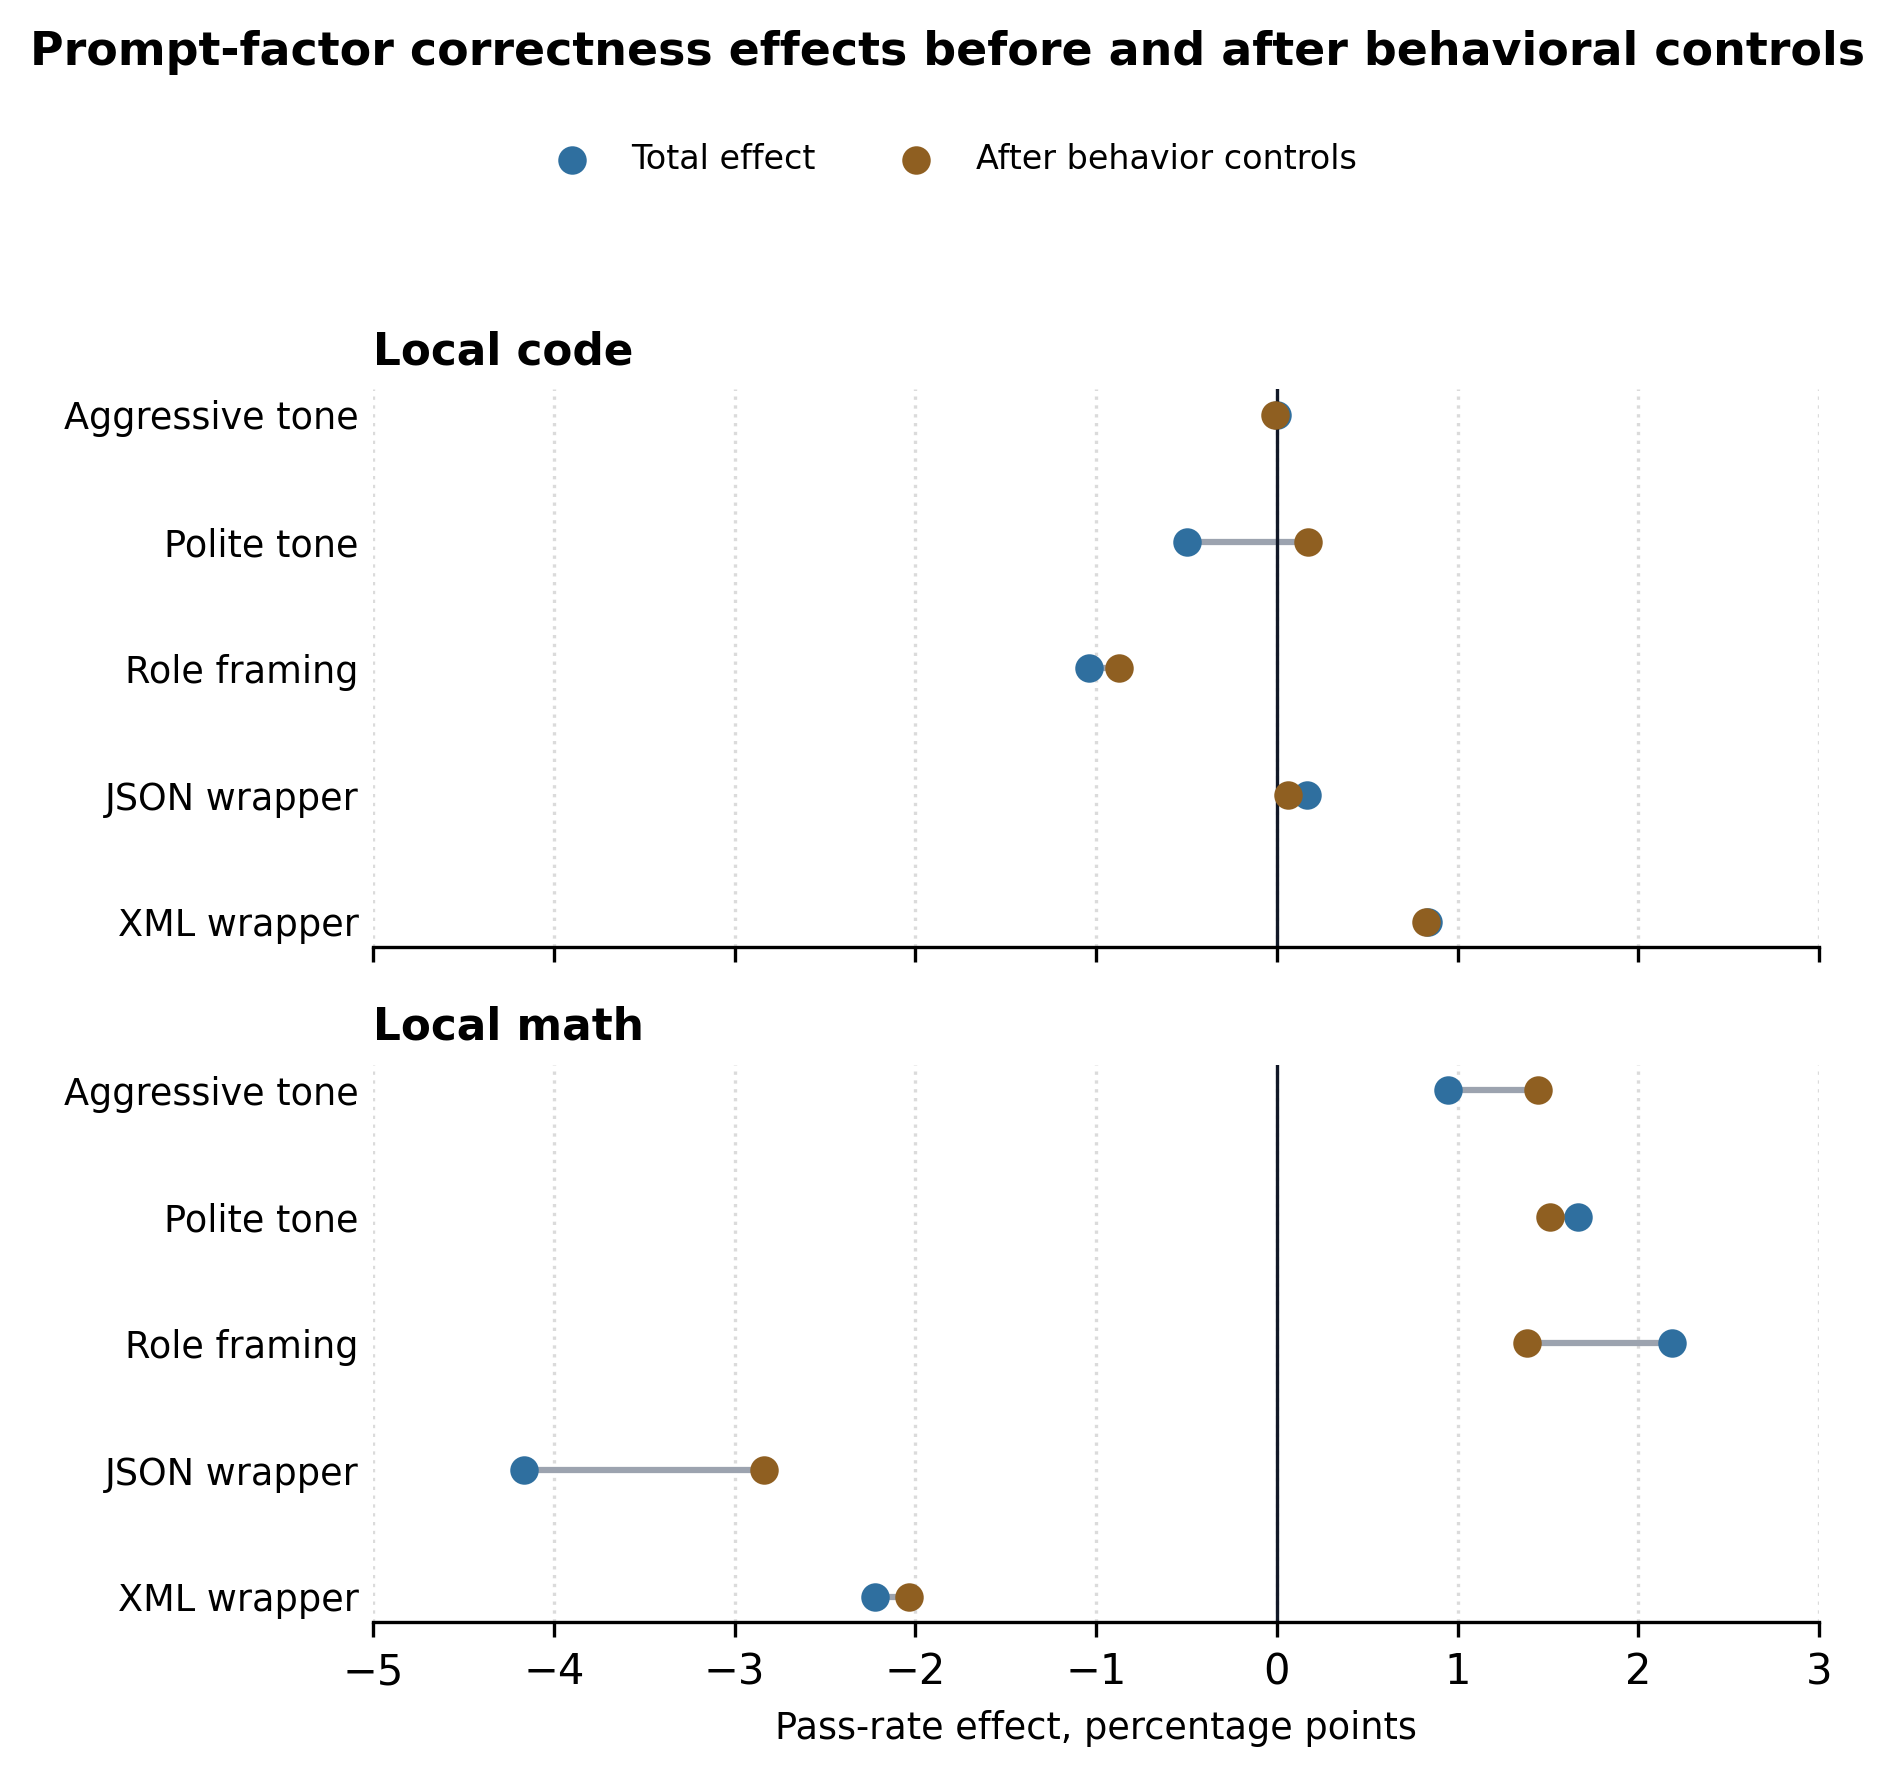
\includegraphics[width=0.95\linewidth,height=\textheight,keepaspectratio,alt={Prompt-factor correctness effects before and after controlling for completion tokens, result-only compliance, and duration.}]{figures/mediation_controls.png}
\caption{Prompt-factor correctness effects before and after controlling for completion tokens, result-only compliance, and duration.}
\label{fig:mediation-controls}
\end{figure}

\begin{longtable}[]{@{}lrr@{}}
\caption{Local code correctness contrasts before and after adjustment for measured behavioral variables.}\label{tab:local-code-mediation}\tabularnewline
\toprule\noalign{}
Local code factor & Total contrast & After behavioral adjustment \\
\midrule\noalign{}
\endfirsthead
\toprule\noalign{}
Local code factor & Total contrast & After behavioral adjustment \\
\midrule\noalign{}
\endhead
\bottomrule\noalign{}
\endlastfoot
Aggressive tone & -0.00 pp & -0.01 pp \\
Polite tone & -0.50 pp & +0.17 pp \\
Role framing & -1.04 pp & -0.87 pp \\
JSON wrapper & +0.17 pp & +0.06 pp \\
XML wrapper & +0.83 pp & +0.82 pp \\
\end{longtable}

For math tasks, the JSON coefficient remains negative after adjustment. The total contrast is -4.17 percentage points; after adjustment for token amount, result-only compliance, and duration, the remaining coefficient is -2.84 percentage points. The measured behaviors are therefore associated with part of the observed contrast, but not all of it. This pattern indicates that JSON-style framing is associated with both the model's observable behavior and downstream correctness in this setting; it should not be interpreted as evidence about the model's hidden reasoning processes.

\begin{longtable}[]{@{}lrr@{}}
\caption{Local math correctness contrasts before and after adjustment for measured behavioral variables.}\label{tab:local-math-mediation}\tabularnewline
\toprule\noalign{}
Local math factor & Total contrast & After behavioral adjustment \\
\midrule\noalign{}
\endfirsthead
\toprule\noalign{}
Local math factor & Total contrast & After behavioral adjustment \\
\midrule\noalign{}
\endhead
\bottomrule\noalign{}
\endlastfoot
Aggressive tone & +0.94 pp & +1.45 pp \\
Polite tone & +1.67 pp & +1.51 pp \\
Role framing & +2.19 pp & +1.38 pp \\
JSON wrapper & -4.17 pp & -2.84 pp \\
XML wrapper & -2.22 pp & -2.04 pp \\
\end{longtable}

Thus, the mediation-style tables serve primarily as associational checkpoints and should not be viewed as a replacement for correctness results or as proof of a mechanism. For local code, the attenuated tone and role coefficients are consistent with a pipeline explanation in which tone and role framing mainly relate to verbosity and ease of parsing. For local math, the measured behavior variables account for only part of the JSON penalty. This residual negative coefficient should be viewed with caution; however, it is exactly the type of outcome that justifies validating prompt policies per task and model rather than trusting universal advice.

\section{Clustered Linear-Probability Robustness Check\label{sec:lpm-robustness}}

As a robustness check on the mixed-effects results, we fit pass/fail linear probability models separately by model group and task type, with prompt factors and model fixed effects and standard errors clustered by base task. The clustered LPM addresses the same repeated-task dependence as the mixed model with a different set of assumptions, and it does not deviate significantly from the main results while correcting for the repetition of the same 50 base tasks across all prompt variants and models.

In the clustered analysis, the core direction of headline effects remains stable and agrees with the mixed-effects model. For API Python, XML stays significant at +4.83 percentage points (clustered SE 1.77, p=0.006), while JSON is positive but marginal at +3.17 percentage points (clustered SE 1.73, p=0.068). For local math, JSON stands at -4.17 percentage points (clustered SE 1.11, p \textless{} 0.001) and XML remains negative at -2.22 percentage points (clustered SE 1.02, p=0.030). Local math role framing is positive at +2.19 percentage points (clustered SE 0.69, p=0.002), and polite tone is also positive at +1.67 percentage points (clustered SE 0.79, p=0.035).

The clustered check sharpens the key narrative instead of reversing it. For positive results, the most robust format is API Python XML, while the most robust negative format is local math JSON. Every effect that is significant in the mixed-effects model is directionally consistent in the clustered LPM, and the remaining effects are either small, model-dependent, or exploratory.

\section{Dominant-Model Sensitivity and Aggregation Risk\label{sec:dominant-sensitivity}}

A single dominant model can overshadow the pooled averages. Removing Nemotron leads to a drop in the local math pass rate from 31.1\% to 19.1\%. The API math pass rate drops by almost half, from 53.3\% to 24.1\%, when DeepSeek V4 Flash is removed. API Python is more stable because Gemini Flash has a similar Python pass rate to DeepSeek V4 Flash. The sensitivity of pooled pass rates to removing dominant models is detailed in Table~\ref{tab:dominant-sensitivity}.

\begin{longtable}[]{@{}llrr@{}}
\caption{Dominant-model sensitivity of pooled pass rates.}\label{tab:dominant-sensitivity}\tabularnewline
\toprule\noalign{}
Sensitivity dataset & Task kind & Full avg. & Without dominant \\
\midrule\noalign{}
\endfirsthead
\toprule\noalign{}
Sensitivity dataset & Task kind & Full avg. & Without dominant \\
\midrule\noalign{}
\endhead
\bottomrule\noalign{}
\endlastfoot
Local, no Nemotron & code & 9.1\% & 6.4\% \\
Local, no Nemotron & math & 31.1\% & 19.1\% \\
API, no DeepSeek & math & 53.3\% & 24.1\% \\
API, no DeepSeek & python & 67.8\% & 69.0\% \\
\end{longtable}

Pass-rate averages, however, do not show whether the prompt effects themselves are distorted by the dominant model. We therefore re-estimated every main tone, role, and format contrast with and without the dominant model in each group, using both the clustered LPM and the mixed-effects logistic model. Table~\ref{tab:dominant-effects} reports the percentage-point effects in both panels; for the API group, the leave-one-out panel contains only Gemini Flash, so those columns are single-model estimates.

{\small
\setlength{\tabcolsep}{3.5pt}
\begin{longtable}[]{@{}llrrrr@{}}
\caption{Prompt-factor effects with and without the dominant model: clustered-LPM percentage-point contrasts and mixed-effects average marginal effects (AME pp).}\label{tab:dominant-effects}\tabularnewline
\toprule\noalign{}
Stratum & Contrast & LPM full & LPM w/o dom. & AME full & AME w/o dom. \\
\midrule\noalign{}
\endfirsthead
\toprule\noalign{}
Stratum & Contrast & LPM full & LPM w/o dom. & AME full & AME w/o dom. \\
\midrule\noalign{}
\endhead
\bottomrule\noalign{}
\endlastfoot
API Python & JSON wrapper & +3.2 & +1.3 & +3.4 & +1.6 \\
API Python & XML wrapper & +4.8 & +2.7 & +5.3 & +3.1 \\
API math & Role framing & -2.8 & -2.4 & -2.8 & -4.1 \\
API math & JSON wrapper & -1.3 & -3.7 & -1.3 & -6.1 \\
API math & XML wrapper & -2.3 & -0.0 & -2.4 & -0.2 \\
Local code & Role framing & -1.0 & -0.9 & -1.0 & -0.9 \\
Local math & Polite tone & +1.7 & +2.3 & +1.6 & +2.3 \\
Local math & Role framing & +2.2 & +2.4 & +2.1 & +2.3 \\
Local math & JSON wrapper & -4.2 & -5.3 & -4.1 & -5.2 \\
Local math & XML wrapper & -2.2 & -2.5 & -2.2 & -2.4 \\
\end{longtable}
}

The re-estimations indicate that the local prompt effects are not merely an artifact of Nemotron's dominance. In the absence of Nemotron, the local math JSON penalty has a slightly greater impact (-5.2 pp AME compared to -4.1 pp in the full panel) while still being highly statistically significant, and the two local math prompt gains (role framing and politeness) exhibit no observable change in their magnitude. Finally, even the small local-code role penalty is just as consistent between both estimates (-0.9 pp AME). Overall, while the leading local model shifts the pooled pass rate by 12 points, it leaves the prompt-effect estimates intact in both direction and magnitude.

The API group displays a different pattern, as expected in a two-model panel. The benefit of the API Python structured format shrinks with the removal of DeepSeek V4 Flash, causing the XML effect to fall from +5.3 to +3.1 pp AME and the JSON effect to decrease from +3.4 to +1.6 pp AME, and neither is shown to be statistically significant in a Gemini-only panel. Therefore, the combined API Python effect must be interpreted as a two-model average with the major input from DeepSeek, and not a feature attributable to each model. The API math role-framing penalty, on the contrary, still holds and becomes even greater in the Gemini-only panel (-4.1 pp AME), which means that it does not depend solely on DeepSeek. The API math XML penalty does not remain after the removal (-0.2 pp AME), thus emphasizing its exploratory character.

This sensitivity test lends support to the primary methodological point: that prompt-policy conclusions must not come from pooled averages only, but be derived from each model group and task type, with the dominant-model dependence of each effect stated explicitly.

Given the unusually high local math pass rate of 91.2\%, Nemotron underwent an independent repository audit. The audited Nemotron math file consists of 900 distinct runs, balanced across 50 base tasks and 18 prompt variants, with zero duplicate task IDs. Since re-computing the pass/fail scores using \texttt{expected\_answer} and \texttt{extracted\_values} reproduced 821 out of 900 passes with zero mismatches against the stored \texttt{passed} field, and a scan found no expected-answer leakage, it is fair to say that the high score is stable across each prompt variant. This figure further demonstrates that the value in question can be treated as a real result, thus justifying the no-Nemotron sensitivity check.

To illuminate the 91.2\% figure at the task level, we provide a breakdown of how the 50 local math tasks perform across the 18 different prompt conditions tested by Nemotron. As shown in Table~\ref{tab:nemotron-task-summary}, the high pass rate is not due to just a few lucky task variants; 42 of the 50 tasks pass in all 18 conditions, 6 tasks pass under some conditions, and only 2 tasks fail in all conditions. Thus, the high average reflects a model that consistently solves most of the task set across various framing conditions, rather than being a mere evaluation artifact affecting a small number of conditions.

\begin{longtable}[]{@{}lr@{}}
\caption{Nemotron 3 Nano local math: task-level solve pattern across the 18 prompt conditions (50 base tasks).}\label{tab:nemotron-task-summary}\tabularnewline
\toprule\noalign{}
Solve pattern across 18 prompt conditions & Number of tasks (of 50) \\
\midrule\noalign{}
\endfirsthead
\toprule\noalign{}
Solve pattern across 18 prompt conditions & Number of tasks (of 50) \\
\midrule\noalign{}
\endhead
\bottomrule\noalign{}
\endlastfoot
Solved under all 18 conditions & 42 \\
Solved under some conditions (1--17) & 6 \\
Solved under no condition & 2 \\
\end{longtable}

\section{Error and Failure Modes\label{sec:failure-modes}}

The experiment shows some of the possible failure modes. Regarding code-based tasks, a few of these failures include wrong algorithms, mistakes in syntax, missing functions, or even outputs incorporating prose or markdown that the extractor cannot cleanly process. The use of both polite and role prompts may lead to parsing issues since they can lead to more explanatory text. Formats such as JSON and XML may make outputs more compact, but they do not guarantee correctness.
The types of failures in math tasks include wrong answers, missing final-answer markers, too brief or vague answers, and extraction ambiguity. Using JSON reduces the duration and length of local math responses while decreasing the pass rate, suggesting that using compact formatting can lower accuracy in certain reasoning tasks even if the requested output is final-result-only. This does not mean that showing reasoning is always required; rather, the results show that less verbose responses are associated with lower local math accuracy in this study.
Representative cases demonstrate the contrast between task-related failures and parser or interface failures. In one Nemotron code run, the response returned by the model was empty, leading to the evaluation of \texttt{No code extracted}. In a different incident with Qwen 2.5, Python code was executed; however, the model used helper names that did not satisfy the requirements of the callable interface, due to which the code execution failed with name-resolution errors. One more instance occurred when a local math run was conducted with Qwen 2.5 using the JSON-format prompt. The result was that the answer \texttt{6} was given when the expected answer was \texttt{12}, showing the compact nature of the answer, which was easily extractable yet erroneous. These examples support the broader interpretation that correctness, extraction compatibility, and output behavior should be reported separately.
